\chapter{Условие}%
\label{cha:uslovie}

Для локальной общей сети был выделен частный адрес:

\textbf{192.168.14.0/24}

\begin{enumerate}
    \item 
        Разделить сеть на 5 подсетей:
        \begin{itemize}
            \item 
                Подсети 1 и 5 должны поддерживать до 14 + 10 устройств
            \item 
                Подсети 2 и 4 должны поддерживать до 5 устройств
            \item 
                Подсеть 3 должна поддерживать только 2 устройства
        \end{itemize}

    \item 
        Настроить DHCP-сервера для выдачи адресов
        \begin{itemize}
            \item 
                Для подсети 1 настроить отдельный DHCP сервер
            \item 
                Для подсети 2 настроить в качестве DHCP-сервера маршрутизатор 1
            \item 
                 Для подсетей 4 и 5 настроить в качестве DHCP-сервера маршрутизатор 2
        \end{itemize}
\end{enumerate}

\chapter{Практическая часть}%
\label{cha:prakticheskaia_chast_}

Практическая часть разделяется на две секции~--- разбиения сети на подсети и настройку DHCP-серверов.

\section{Разбиение сети на подсети}%
\label{sec:razbienie_seti_na_podseti}

\begin{table}[H]
\centering
\caption{Подсети}
\label{tbl:subnets}
\begin{tabular}{|r|>{\raggedleft}p{2cm}|l|>{\raggedleft}p{2cm}|>{\raggedleft}p{3cm}|r|}
    \hline
    \textnumero{} & Кол-во хостов & Адрес подсети & Диапазон адресов & Широко-вещательный & Маска \\
    \hline
    1 & 30 & 192.168.14.0  &  0-31 & 31 & 27 \\
    \hline
    2 &  6 & 192.168.14.64 & 64-71 & 71 & 29 \\
    \hline
    3 &  2 & 192.168.14.80 & 80-83 & 83 & 30 \\
    \hline
    4 &  6 & 192.168.14.72 & 72-79 & 79 & 29 \\
    \hline
    5 & 30 & 192.168.14.32 & 32-63 & 63 & 27 \\
    \hline
    \end{tabular}
\end{table}

В таблице~\ref{tbl:subnets} приведены только хостовые части адресов в столбцах <<Диапазон адресов>> и <<Широковещательный>>, маска указана в нотации CIDR.

\section{Настройка DHCP-серверов}%
\label{sec:nastroika_dhcp_serverov}

На рисунке~\ref{fig:servers1} представлена настройка DHCP-сервера для первой подсети.

\begin{figure}[H]
    \centering
    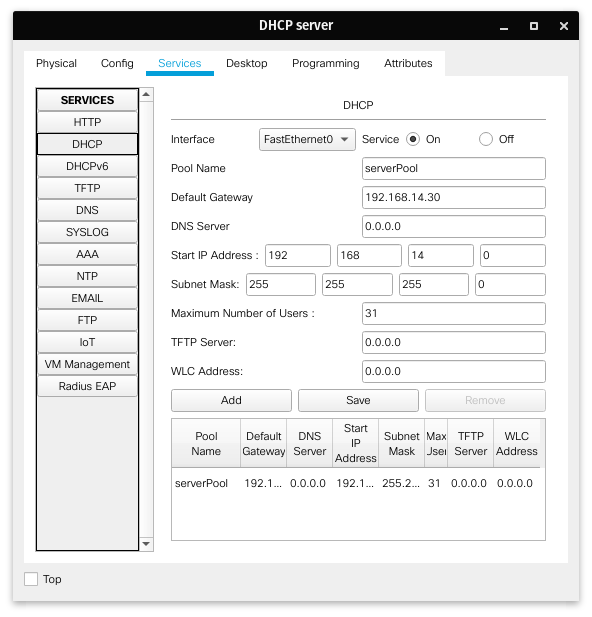
\includegraphics[width=0.8\linewidth]{images/src01.png}
    \caption{Настройка сервера для первой подсети}%
    \label{fig:servers1}
\end{figure}

\lstset{
    language=bash
}

Для настройки маршрутизатора в качестве DHCP-сервера для второй подсети были использованы команды:
\begin{lstlisting}[caption={Команды для настройки второй подсети}]
ip dhcp pool subnet2
network 192.168.14.64 255.255.255.248
default-router 192.168.14.70
\end{lstlisting}

\begin{figure}[H]
    \centering
    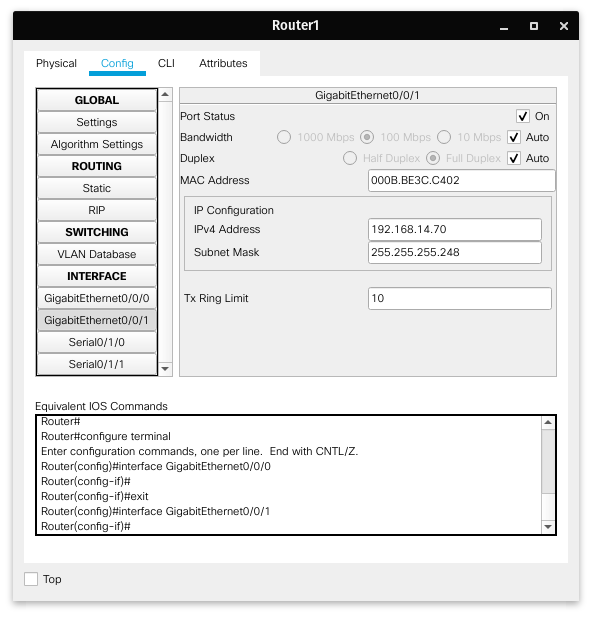
\includegraphics[width=0.8\linewidth]{images/src02.png}
    \caption{Настройка маршрутизатора для второй подсети}%
    \label{fig:servers2}
\end{figure}

Адреса выдаются автоматически исходя из диапазона сетей подсети \textnumero2.

Для третьей подсети маршрутизаторы были настроены следующим образом:
\begin{figure}[H]
    \centering
    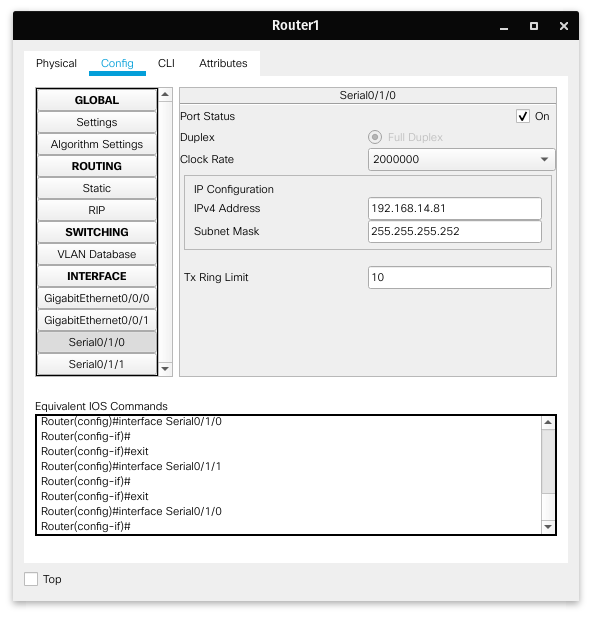
\includegraphics[width=0.8\linewidth]{images/src03.png}
    \caption{Настройка первого маршрутизатора для третьей подсети}%
    \label{fig:servers3_1}
\end{figure}
\begin{figure}[H]
    \centering
    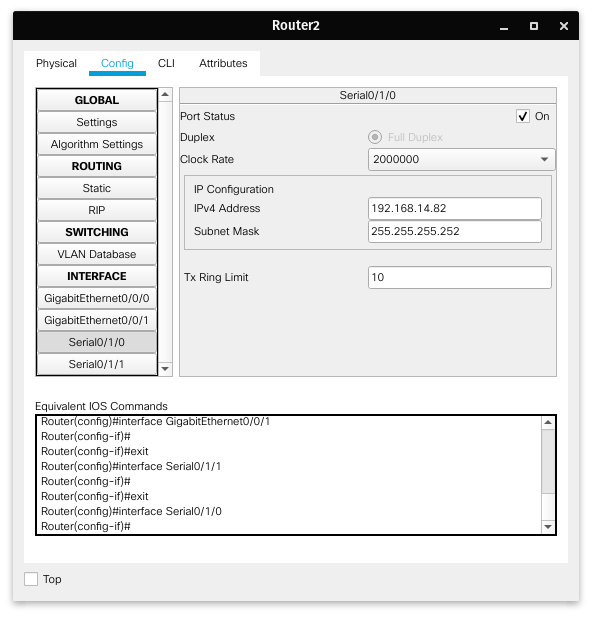
\includegraphics[width=0.8\linewidth]{images/src04.png}
    \caption{Настройка второго маршрутизатора для третьей подсети}%
    \label{fig:servers3_2}
\end{figure}

Для настройки маршрутизатора в качестве DHCP-сервера для четвёртой подсети были использованы команды:
\begin{lstlisting}[caption={Команды для настройки четвёртой подсети}]
ip dhcp pool subnet4
network 192.168.14.72 255.255.255.248
default-router 192.168.14.78
\end{lstlisting}

\begin{figure}[H]
    \centering
    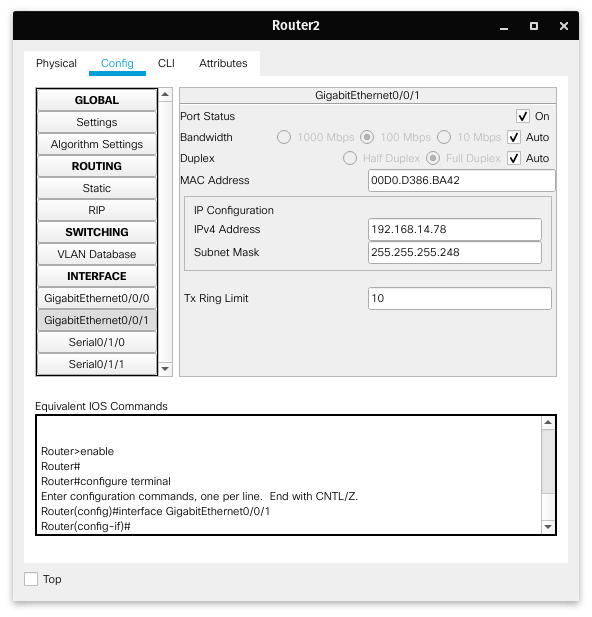
\includegraphics[width=0.8\linewidth]{images/src05.png}
    \caption{Настройка маршрутизатора для четвёртой подсети}%
    \label{fig:servers4}
\end{figure}

Адреса выдаются автоматически исходя из диапазона сетей подсети \textnumero4.

Для настройки маршрутизатора в качестве DHCP-сервера для пятой подсети были использованы команды:
\begin{lstlisting}[caption={Команды для настройки пятой подсети}]
ip dhcp pool subnet5
network 192.168.14.32 255.255.255.224
default-router 192.168.14.62
\end{lstlisting}

\begin{figure}[H]
    \centering
    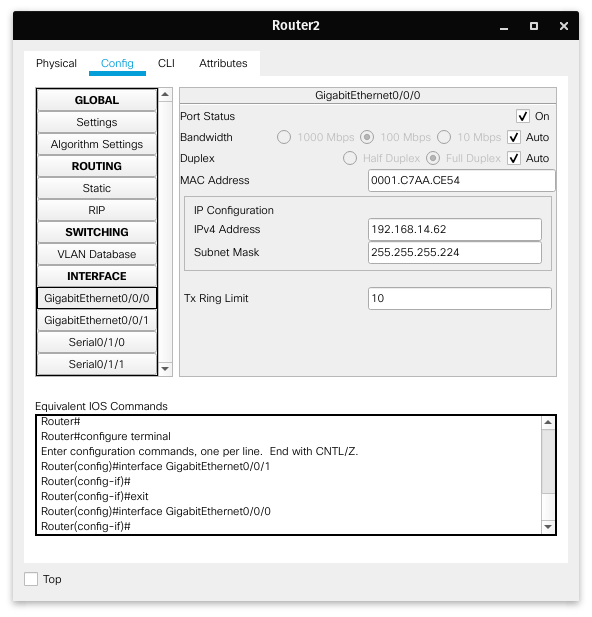
\includegraphics[width=0.8\linewidth]{images/src06.png}
    \caption{Настройка маршрутизатора для пятой подсети}%
    \label{fig:servers5}
\end{figure}

Адреса выдаются автоматически исходя из диапазона сетей подсети \textnumero5.

\subsection{Проверка работы}%
\label{sub:proverka_raboty}

Продемонстрируем успешное выполнение команды ping внутри пятой подсети:
\begin{figure}[H]
    \centering
    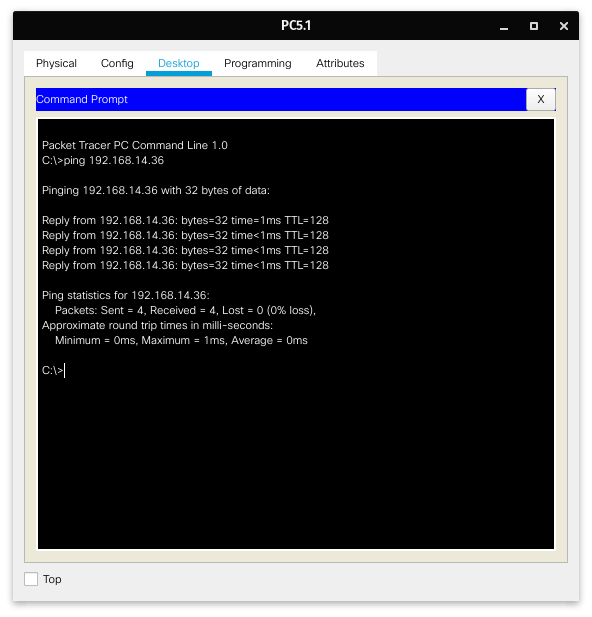
\includegraphics[width=0.8\linewidth]{images/src07.png}
\end{figure}


Продемонстрируем неудачное выполнение команды ping при обращении из первой подсети к пятой:
\begin{figure}[H]
    \centering
    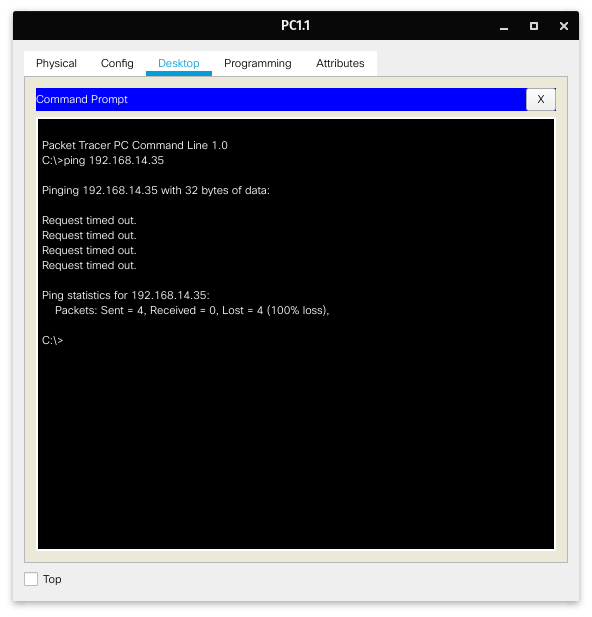
\includegraphics[width=0.8\linewidth]{images/src08.png}
\end{figure}

\chapter{Вывод}%
\label{cha:vyvod}

Таким образом, в результате выполнения данной лабораторной работы были выполнены поставленные задачи: сеть была разделена на 5 подсетей; настроены DHCP-сервера для выдачи адресов. Так же была выполнена проверка работоспособности сети.
